\chapter{Higher order methods I: the Runge-Kutta family}

So far in the course we have mostly focused on 
the forward and backward Euler methods both of 
which are first order consistent and convergent. We typically 
just say that these methods are first order accurate to mean 
that their local truncation and global errors are 
$\mathcal{O}(\Delta t)$. While these methods are simple and easy 
to understand, in practice we often would like to use more accurate 
methods, ideally those who have accuracy $\mathcal{O}(\Delta t^p)$ 
for $p=2$ or $p=4$. Let's say we come up with a second order method, 
i.e., $p=2$. Then by halving the stepm size $\Delta t \leftarrow \frac{\Delta t}{2}$, the error should decrease by a factor of $2^2 = 4$. If the method 
is fourth order, i.e., $p=4$ then the error will drop by 
a factor of $16$! Thus, pursuing such methods can realyl pay off in practice. 

In this lecture we will consider one approach to the design of such methods 
that is often called a one-step method: these are 
update schemes where $\ub_{n}$ is computed only from $\ub_{n-1}$. In 
the next example we will introduce multi-step methods where $\ub_{n}$ 
is computed using multiple previous values such as 
$\ub_{n-1}, \ub_{n-2}, \dots, \ub_{n-k}$ for some $k \ge 1$.


\section{From quadrature to Runge-Kutta methods}

Our starting point in deriving higher order methods is 
the approximation of integrals, which is called 
quadrature. Broadly speaking, consider some function 
$g:[a, b] \to \R$ and suppose we want to approximate 
\begin{equation*}
    \int_a^b g(x) \, dx.
\end{equation*}
In quadrature we consider $s$ distinct points $x_1, x_2, \dots, x_s \in [a, b]$ and corresponding weights $w_1, w_2, \dots, w_s$ to approximate the integral as
\begin{equation*}
    \sum_{i=1}^s w_i g(x_i) \approx \int_{a}^{b} g(x) \, dx.
\end{equation*}
The choice of the weights and points $(x_i, w_i)$ constitutes 
the quadrature rule. Popular examples are: 
\begin{equation*}
    \begin{aligned}[t]
        \text{left point rule:} & \quad \int_a^b g(x) \, dx \approx (b-a) g(a), \\
        \text{right point rule:} & \quad \int_a^b g(x) \, dx \approx (b-a) g(b), \\
        \text{midpoint rule:} & \quad \int_a^b g(x) \, dx \approx (b-a) g\Big(\frac{a+b}{2}\Big), \\
        \text{trapezoidal rule:} & \quad \int_a^b g(x) \, dx \approx \frac{b-a}{2} \Big(g(a) + g(b)\Big)
    \end{aligned}
\end{equation*}
These rules are illustrated in \Cref{fig:quadrature-rules}.

\begin{figure}[htp]
    \centering
    \begin{tikzpicture}[thick, scale=0.9,
        declare function={g(\x) = 0.8 + 0.5*\x + 0.4*sin(deg(2*\x)); xa = 0.5; xb = 3; xm = 1.75;},
        area/.style={fill=blue!20, draw=blue!70!black},
        dot/.style={circle, fill, inner sep=1.5pt}]
        % axes, the function g, and labels common to all panels
        \newcommand{\quadpanel}[1]{
            \draw[->] (0,0) -- (4,0) node[right] {$x$};
            \draw[->] (0,0) -- (0,3) node[above] {$y$};
            \draw[very thick, domain=0.1:3.6, samples=100, smooth] plot (\x,{g(\x)}) node[right] {$g(x)$};
            \node[below] at (xa,0) {\strut$a$};
            \node[below] at (xb,0) {\strut$b$};
            \node at (2,-1.1) {#1};
        }

        % left point rule
        \begin{scope}[shift={(0,5)}]
            \draw[area] (xa,0) rectangle (xb,{g(xa)});
            \quadpanel{left point rule}
            \node[dot] at (xa,{g(xa)}) {};
        \end{scope}

        % right point rule
        \begin{scope}[shift={(6,5)}]
            \draw[area] (xa,0) rectangle (xb,{g(xb)});
            \quadpanel{right point rule}
            \node[dot] at (xb,{g(xb)}) {};
        \end{scope}

        % midpoint rule
        \begin{scope}[shift={(0,0)}]
            \draw[area] (xa,0) rectangle (xb,{g(xm)});
            \draw[dashed, thin] (xm,0) -- (xm,{g(xm)});
            \quadpanel{midpoint rule}
            \node[below] at (xm,0) {$\frac{a+b}{2}$};
            \node[dot] at (xm,{g(xm)}) {};
        \end{scope}

        % trapezoidal rule
        \begin{scope}[shift={(6,0)}]
            \draw[area] (xa,0) -- (xa,{g(xa)}) -- (xb,{g(xb)}) -- (xb,0) -- cycle;
            \quadpanel{trapezoidal rule}
            \node[dot] at (xa,{g(xa)}) {};
            \node[dot] at (xb,{g(xb)}) {};
        \end{scope}
    \end{tikzpicture}
    \caption{The left point, right point, midpoint, and trapezoidal rules 
    applied to a smooth function $g$ on $[a, b]$. The shaded region in 
    each panel is the area computed by the quadrature rule, while the 
    exact integral is the area under the curve $g(x)$. Black dots mark 
    the points where $g$ is evaluated.}
    \label{fig:quadrature-rules}
\end{figure}

Let us now consider a generic scalar valued ODE 
\begin{equation*}
    u' = f(t,u), 
\end{equation*}
where we switched to the standard prime notation 
$u'(t) = \frac{d u}{dt}(t)$ for convenience.
We will develop our methods for this case but note that 
they have a natural extension to systems of ODEs that 
we will discuss later. 

Consider the interval $[t_{n-1}, t_n]$ and integrate both sides of the ODE:
\begin{equation*}
    u(t_n) - u(t_{n-1}) = 
    \int_{t_{n-1}}^{t_n} u'(t) \, dt.
\end{equation*}
Let us now approximate the integral on the 
right hand side using the left point rule: 
\begin{equation*}
    u(t_n) - u(t_{n-1}) \approx (t_n - t_{n-1}) u'(t_{n-1}) 
    = \Delta t \, f(t_{n-1}, u(t_{n-1})),
\end{equation*}
which gives rise to the explicit scheme 
\begin{equation*}
    u_n = u_{n-1} + \Delta t f(t_{n-1}, u_{n-1})
\end{equation*}
which we recognize as the forward Euler scheme. Using the 
right point rule we obtain backward Euler:
\begin{equation*}
    u(t_n) - u(t_{n-1}) \approx \Delta t u'(t_n) 
    = \Delta t f(t_n, u(t_n)) 
\end{equation*}
which gives rise to the implicit scheme 
\begin{equation*}
    u_n = u_{n-1} + \Delta t f(t_n, u_n)
\end{equation*}
which is simply the backward Euler scheme. 
Continuing forward, if we use the midpoint rule we 
obtain the expression
\begin{equation*}
    \begin{aligned}
    u(t_n) - u(t_{n-1}) &\approx 
    \Delta t u'\Big(\frac{t_{n-1}+t_n}{2}\Big) 
    = \Delta t f\Big(\frac{t_{n-1}+t_n}{2}, u\Big(\frac{t_{n-1}+t_n}{2}\Big)\Big).
    \end{aligned}
\end{equation*}
Now if we approximate $u\Big(\frac{t_{n-1}+t_n}{2}\Big)$ 
by the average of $u(t_{n-1})$ and $u(t_n)$, 
we obtain the implicit midpoint scheme 
\begin{equation*}
    u_n = u_{n-1} + \Delta t f \Big( t_{n- \frac12}, \frac{u_n + u_{n-1}}{2} \Big).
\end{equation*}
Alternatively, we can construct an explicit midpoint method 
by approximating $u(\frac{t_{n-1} + t_n}{2})$ 
using an intermediate forward Euler step to obtain 
\begin{equation}\label{eq:explicit-midpoint}
    \begin{aligned}
    \hat{u}_{n-1/2} &= u_{n-1} + \frac{\Delta t}{2} f(t_{n-1}, u_{n-1}),\\
    u_n &= u_{n-1} + \Delta t f\Big(t_{n- \frac12}, \hat{u}_{n-1/2}\Big).
    \end{aligned}
\end{equation}
The explicit midpoint method above is our first example of a 
Runge-Kutta method: {\it the idea is to construct a series 
of intermediate approximations to the solution at each 
step in order to improve the order of accuracy.}
The explicit midpoint method above is sometimes also 
called an RK2 method. The reason for doing 
this additional step is that the resulting 
explicit scheme turns out to be second order accurate:

To see this, consider 
the local truncation error
\begin{equation*}
\begin{aligned}
    \tau_n & = \frac{u(t_n) - u(t_{n-1})}{\Delta t} - f\Big(t_{n- \frac12}, \hat{u}_{n-1/2}\Big) \\ 
    & = u'(t_n) + \frac{\Delta t}{2} u''(t_n) + \frac{\Delta t^2}{8} u'''
    - \Big( 
    f(t_n, u(t_n)) + \frac{\Delta t}{2} 
    [ \partial_t f(t_n, u(t_n)) + \partial_u f(t_n, u(t_n)) u'(t_n) ] 
    \\ 
    & \qquad + \frac{\Delta t^2}{8} 
    [ \partial_{tt} f(t_n, u(t_n)) 
    + 2 \partial_{tu} f(t_n, u(t_n)) u'(t_n) 
    + \partial_{uu} f(t_n, u(t_n)) (u'(t_n))^2 ]
    \Big) + \mathcal{O}(\Delta t^3) \\
    & = u'(t_n) + \frac{\Delta t}{2} u''(t_n) 
    + \frac{\Delta t^2}{8} u'''
    - \Big( 
    f(t_n, u(t_n)) + \frac{\Delta t}{2} 
    [ \partial_t f(t_n, u(t_n))
     + \partial_u f(t_n, u(t_n)) f(t_n, u(t_n)) ] 
    \\ 
    & \qquad + \frac{\Delta t^2}{8} 
    [ \partial_{tt} f(t_n, u(t_n)) 
    + 2 \partial_{tu} f(t_n, u(t_n)) f(t_n, u(t_n)) 
    + \partial_{uu} f(t_n, u(t_n)) (f(t_n, u(t_n)))^2 ]
    \Big) \\ 
    & \qquad + \mathcal{O}(\Delta t^3)
\end{aligned} 
\end{equation*}
At the same time by differentiating the ODE we obtain, 
\begin{equation*}
    \begin{aligned}
    u'(t_n) &= f(t_n, u(t_n)), \\
    u''(t_n) &= \partial_t f(t_n, u(t_n)) + \partial_u f(t_n, u(t_n)) u'(t_n), \\
    u'''(t_n) &= \partial_{tt} f(t_n, u(t_n)) 
    + 2 \partial_{tu} f(t_n, u(t_n)) u'(t_n) 
    + \partial_{uu} f(t_n, u(t_n)) (u'(t_n))^2
    + \partial_u f(t_n, u(t_n)) u''(t_n)
    \end{aligned}
\end{equation*}
which, after substitution back into the expression for $\tau_n$ 
reveals that the terms of order $1$, $\Delta t$ cancel 
and we are left with a local truncation error of order 
$\mathcal{O}(\Delta t^2)$. Additionally, it can be shown 
that this method is $0$-stable which, by Lax's theorem, 
gives second-order convergence.

Continuing the same line of thinking, and by using more 
accurate quadrature rules we can design higher order 
Runge-Kutta methods. Among these the most popular scheme 
is the classical fourth-order Runge-Kutta method (RK4) 
which is widely used in off-the-shelf numerical solvers
in scientific computing packages. The scheme takes the 
following form: 
\begin{equation*}
    \begin{aligned}
        \hat{u}_1 & = u_{n-1} \\
        \hat{u}_2 & = u_{n-1} + \frac{\Delta t}{2} f(t_{n-1}, \hat{u}_1)\\
        \hat{u}_3 & = u_{n-1} + \frac{\Delta t}{2} f( t_{n-1/2}, \hat{u}_2) \\
        \hat{u}_4 & = u_{n-1} + \Delta t f( t_{n-1/2}, \hat{u}_3) \\
        u_n & = u_{n-1} + \frac{\Delta t}{6} \Big( f(t_{n-1}, \hat{u}_1) + 2 f(t_{n-1/2}, \hat{u}_2) + 2 f(t_{n-1/2}, \hat{u}_3) + f(t_n, \hat{u}_4) \Big)
    \end{aligned}
\end{equation*}
The resulting scheme is fourth-order accurate which is why it is 
popular in applications where high accuracy is needed. Observe that 
the intermediate values, the $\hat{u}_i$ are simply forward Euler approximations
of the solution computed from our previous estimates for $u_n$ and 
even though forward Euler is only first-order accurate, the 
combination of these estimates ends up being fourth-order accurate. 

Since the above methods are all explicit we expect that they may have 
stability restrictions. In \Cref{fig:RK-stability} we plot 
the regions for forward Euler, the explicit midpoint method, and 
the RK4 scheme. 

\begin{figure}
   \centering
   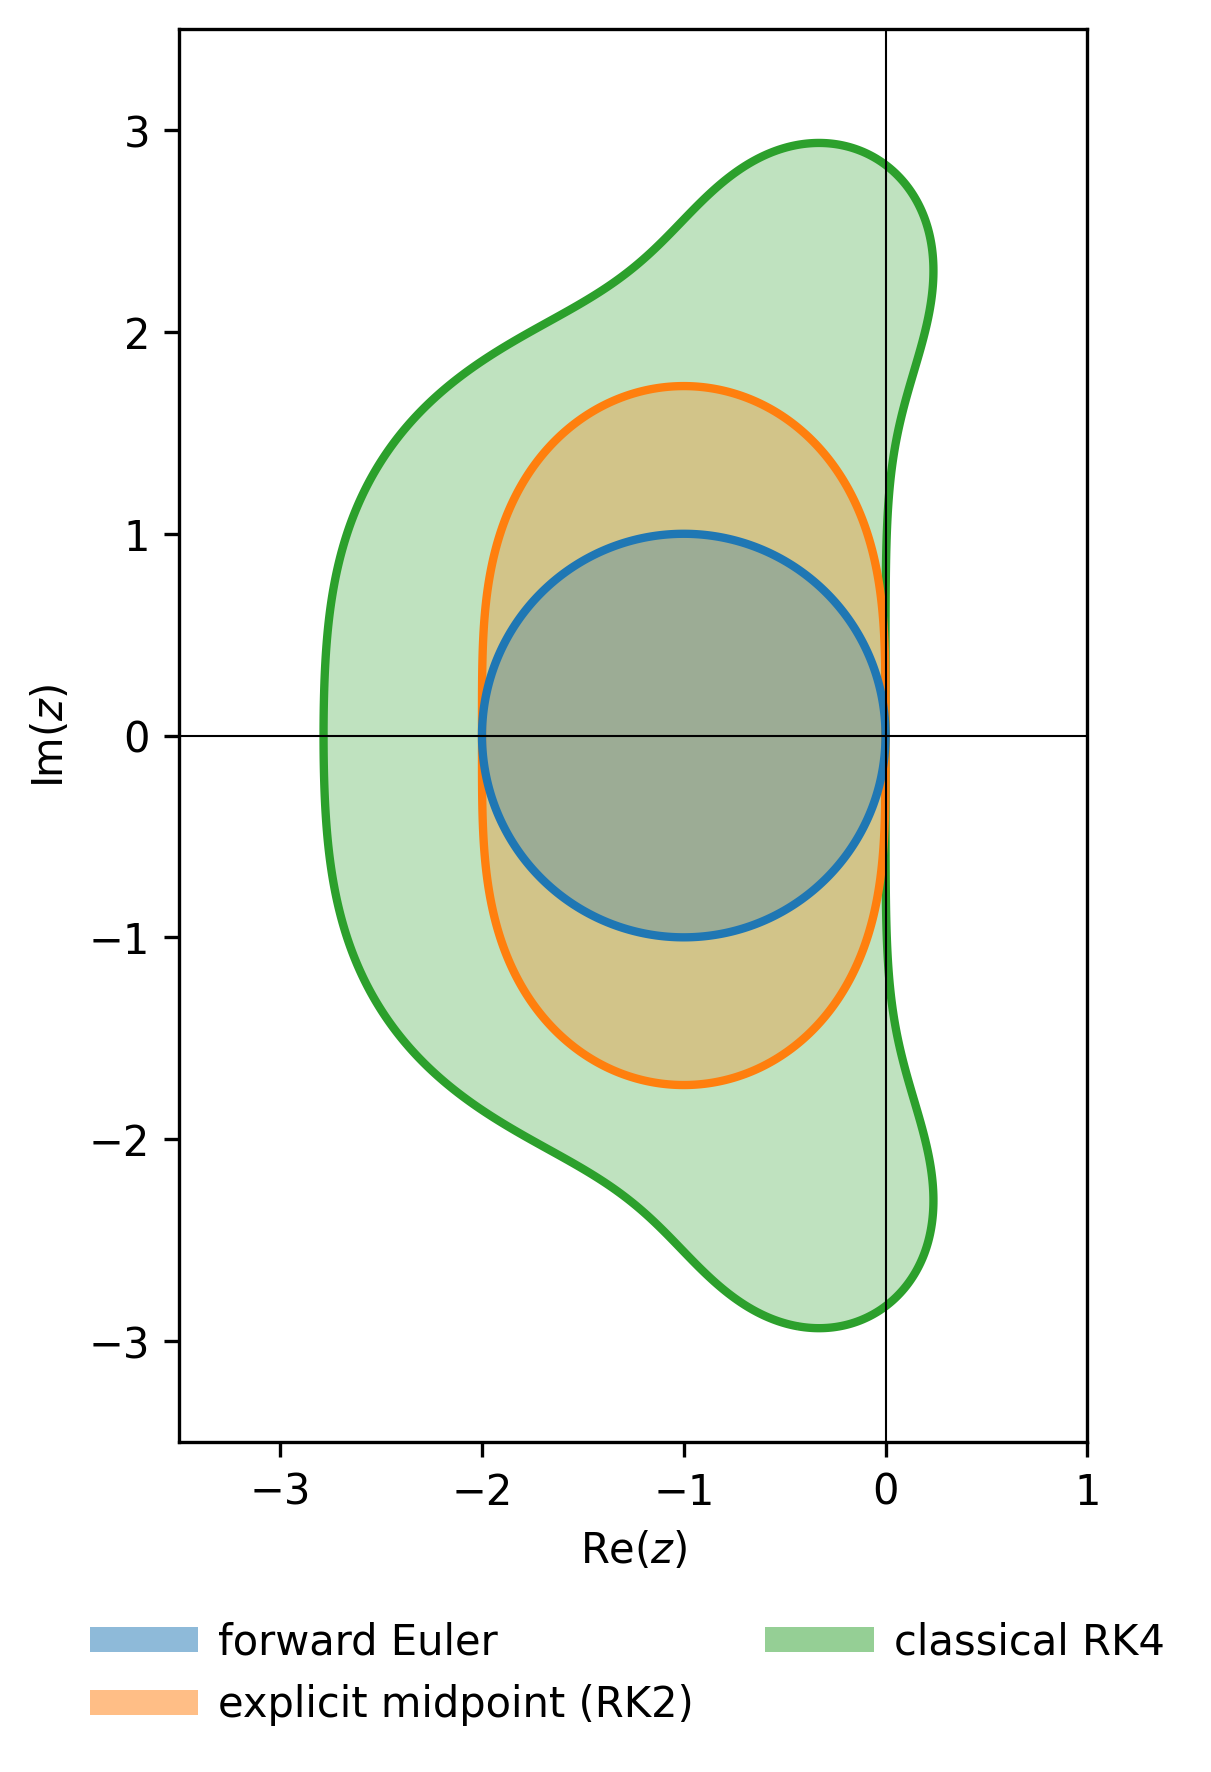
\includegraphics[width=0.6\textwidth]{./Lectures/Lec9/stability_regions_rk.png}
   \caption{Stability regions for various explicit Runge-Kutta methods.}
   \label{fig:RK-stability}
\end{figure}

% \begin{equation*}
%     u(t_n) - u(t_{n-1}) = \int_{t_{n-1}}^{t_n} u'(t) \, dt = \int_{t_{n-1}}^{t_n} f(u(t)) \, dt.
% \end{equation*}



% \bibliographystyle{plainnat}
% \bibliography{references}